\documentclass[12pt, t]{beamer}

%------------------------------------------------------------------------------
% configuration
%------------------------------------------------------------------------------
\RequirePackage{etex}
\usepackage{currfile-abspath}
\usepackage{../../themes/dbt}
\usepackage{catchfilebetweentags}

\setbeameroption{hide notes}
\setbeamertemplate{caption}{\raggedright\insertcaption\par}

\graphicspath{{images/}}
\getmainfile
\getabspath{\themainfile}
\let\mainabsdir\theabsdir
\let\mainabspath\theabspath

\newcommand{\insertcode}[2]{\lstinputlisting[label=samplecode, basicstyle=#1]{\mainabsdir/code/#2}}
\newcommand{\bi}{\begin{itemize}}
\newcommand{\ei}{\end{itemize}}
\newcommand{\ig}{\includegraphics}
\newcommand{\myhref}[1]{\href{#1}{\tt \scriptsize #1}}
\newcommand{\incnote}[1]{\note{\ExecuteMetaData[notes.tex]{#1}}}
\newcommand{\src}[2]{\vspace{-10pt}\caption{\href{#1}{\centering \tt \tiny [#2]}}}


%------------------------------------------------------------------------------
% title
%------------------------------------------------------------------------------
%------------------------------------------------------------------------------
% title
%------------------------------------------------------------------------------
% slide
\title{Systèmes d'exploitation pour l'embarqué}
\subtitle{UV 5.2 - Exécution et Concurrence}

\author{\href{}{Paul Blottière}}
\institute{
    \href{http://www.ensta-bretagne.fr/}{ENSTA Bretagne} \\[2pt]
    \href{}{\tt \scriptsize 2017 / 2018}
}
\date{
    \href{https://github.com/pblottiere}{\tt \scriptsize https://github.com/pblottiere} \\[2pt]
    %\href{blottiere.paul@gmail.com}{\tt \scriptsize blottiere.paul@gmail.com}
}

% info
\begin{document}

{
\setbeamertemplate{footline}{} % no page number here
\frame{
    \titlepage
} }

%------------------------------------------------------------------------------
% amélioration continue
%------------------------------------------------------------------------------
\begin{frame}{Amélioration continue}
    \subt{Contributions}
    \vspace{12pt}

    \begin{center}
    
\includegraphics[scale=0.7]{github.png}
    \end{center}

    \bi
    \itemsep12pt
    \item Dépôt du cours : \href{https://github.com/pblottiere/embsys}{\tt \scriptsize https://github.com/pblottiere/embsys}
    \item Souhaits d'amélioration, erreurs, idées de TP, ... : ouverture d'Issues (avec le bon label!)
    \item Apports de corrections : Pull Request
    \ei
\end{frame}




%<**lecture_content>
%------------------------------------------------------------------------------
% lecture
%------------------------------------------------------------------------------
\begin{frame}[plain,c]
    \centering
    \huge\textcolor{title}{Linux embarqué : compilation et outils}
\end{frame}

%------------------------------------------------------------------------------
% plan
%------------------------------------------------------------------------------
\begin{frame}{Plan}
    \subt{}
    \vspace{8pt}

    \begin{enumerate}
        \itemsep6pt
        \item Autotools et menuconfig
        \item Une distribution minimale
        \item Cross-compilation
        \item Compilation du kernel
        \item Busybox
        \item U-Boot
        \item Automatisation (Buildroot, Yocto Project, ...)
        \item QEMU
    \end{enumerate}

    \note {
    }
\end{frame}

%------------------------------------------------------------------------------
% rec1
%------------------------------------------------------------------------------
\begin{frame}{Autotools et menuconfig (1)}
    \subt{Les autotools}

    \vspace{15pt}
    Ensemble d'outils de build du projet GNU.

    \begin{figure}
        \centering
        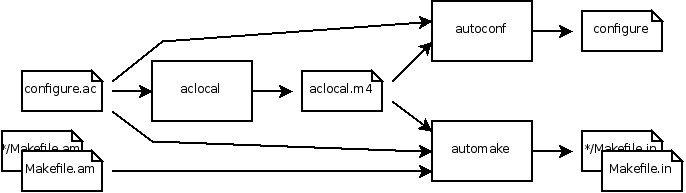
\includegraphics[scale=0.45]{autotools.png}
    \end{figure}

    \onslide<2->
    {
        \vspace{15pt}
        => très utilisé, aux côté de CMake!
    }
\end{frame}

%------------------------------------------------------------------------------
% rec2
%------------------------------------------------------------------------------
\defverbatim{\lstauto}
{
    \begin{lstlisting}
> ./configure
...
> make
...
> sudo make install
...
    \end{lstlisting}
}

\begin{frame}{Autotools et menuconfig (2)}
    \subt{Les autotools}

    \vspace{10pt}
    Utilisation classique sans paramétrage :
    \vspace{5pt}
    \lstauto

    \onslide<2->
    {
        \vspace{10pt}
        => par défaut, l'installation se fera avec le prefix {\textbf{/}} :
        \bi
        \itemsep8pt
        \item /usr/bin
        \item /usr/lib
        \item /usr/share
        \item ...
        \ei
    }
\end{frame}

%------------------------------------------------------------------------------
% rec3
%------------------------------------------------------------------------------
\begin{frame}{Autotools et menuconfig (3)}
    \subt{Les autotools}

    \vspace{10pt}
    La phase de configuration, via l'exécution de {\textit{./configure}},
    prend de nombreux paramètres en entrée :
    \vspace{5pt}
    \bi
    \itemsep8pt
    \item {\textit{- -build}} : système d'exécution courant
    \item {\textit{- -host}} : système où le résultat de la compilation
          sera exécuté
    \item {\textit{- -prefix}} : prefix d'installation utilisé lors du
          {\textit{make install}}
    \item {\textit{- -enable-<FEATURE>}} : active la fonctionnalité
    \item {\textit{- -disable-FEATURE}} : désactive la fonctionnalité
    \item {\textit{- -help}} : affiche la liste des commandes disponibles
    \item ...
    \ei
\end{frame}

%------------------------------------------------------------------------------
% rec4
%------------------------------------------------------------------------------
\defverbatim{\lstconf}
{
    \begin{lstlisting}
> ./configure
checking build system type... x86_64-pc-linux-gnu
checking host system type... x86_64-pc-linux-gnu
...
checking for ncursesw/curses.h... no
checking ncurses.h usability... yes
checking ncurses.h presence... yes
checking for ncurses.h... yes
configure: creating ./config.status
config.status: creating Makefile
    \end{lstlisting}
}

\begin{frame}{Autotools et menuconfig (4)}
    \subt{Les autotools}

    \vspace{15pt}
    Un des rôles du script {\textit{configure}} est de vérifier la présence
    de toutes les dépendances et de construire les Makefile associés à partir
    des Makefile.in

    \onslide<2->
    {
        \vspace{15pt}
        \lstconf
    }
\end{frame}

%------------------------------------------------------------------------------
% rec5
%------------------------------------------------------------------------------
\begin{frame}{Autotools et menuconfig (5)}
    \subt{Menuconfig}

    \vspace{10pt}
    {\textbf{ncurses / New Curses}} : API de développement d'interface graphique
    simple en mode texte et exécutable dans un terminal.

    \onslide<2->
    {
        \vspace{10pt}
        {\textbf{kconfig}} : langage de configuration développé initialement par
        Linus Torvalds pour configurer le kernel à travers une IHM utilisant
        ncurses.
    }

    \onslide<3->
    {
        \vspace{10pt}
        => désormais, kconfig est utilisé par beaucoup d'autre projets de par sa
        légèreté et sa facilité d'utilisation :

        \bi
        \item kernel
        \item busybox
        \item crosstool-ng
        \item cross-builder
        \item ...
        \ei
    }
\end{frame}

%------------------------------------------------------------------------------
% rec6
%------------------------------------------------------------------------------
\defverbatim{\lstmenu}
{
    \begin{lstlisting}
> make menuconfig
    \end{lstlisting}
}

\begin{frame}{Autotools et menuconfig (6)}
    \subt{Menuconfig}

    \vspace{15pt}
    Par héritage, le lancement d'une IHM de configuration utilisant Kconfig se
    fait en exécutant la commande :

    \vspace{5pt}
    \lstmenu

    \onslide<2->
    {
        \begin{figure}
            \centering
            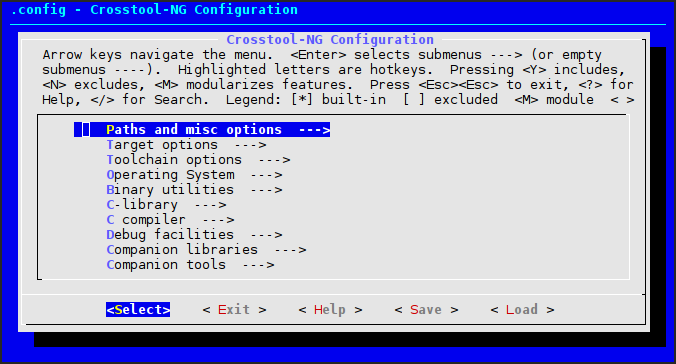
\includegraphics[scale=0.5]{ct-ng.png}
        \end{figure}
    }
\end{frame}

%------------------------------------------------------------------------------
% rec7
%------------------------------------------------------------------------------
\defverbatim{\lstkconf}
{
    \begin{lstlisting}
CONFIG_OID_REGISTRY=m
CONFIG_UCS2_STRING=y
CONFIG_FONT_SUPPORT=y
# CONFIG_FONTS is not set
CONFIG_FONT_8x8=y
CONFIG_FONT_8x16=y
CONFIG_ARCH_HAS_SG_CHAIN=y
CONFIG_ARCH_HAS_PMEM_API=y
    \end{lstlisting}
}

\begin{frame}{Autotools et menuconfig (7)}
    \subt{Menuconfig}

    \vspace{15pt}
    En sortie, un fichier de configuration, utilisé au moment du make, est
    généré à partir des éléments configurés dans l'interface :

    \vspace{10pt}
    \lstkconf

    \onslide<2->
    {
        => il existe souvent des fichiers de configuration prédéfinis pour des
        buts bien particuliers!
    }
\end{frame}

%------------------------------------------------------------------------------
% rec8
%------------------------------------------------------------------------------
\defverbatim{\lstkconf}
{
    \begin{lstlisting}
config MODVERSIONS
	bool "Set version info on module symbols"
	depends on MODULES
	help
        Usually, modules have to be recompiled
        whenever you switch to a new kernel.  ...
    \end{lstlisting}
}

\begin{frame}{Autotools et menuconfig (8)}
    \subt{Menuconfig}

    \vspace{15pt}
    Un exemple de script utilisant le langage KConfig :
    \vspace{5pt}
    \lstkconf
\end{frame}

%------------------------------------------------------------------------------
% mini1
%------------------------------------------------------------------------------
\begin{frame}{Une distribution minimale (1)}
    \subt{Kernel et RFS}

    \vspace{15pt}
    Une distribution minimale basée sur le noyau Linux nécessite seulement
    deux éléments :
    \bi
    \itemsep6pt
    \item un kernel
    \item un RFS contenant les binaires et les librairies de base
    \ei

    \begin{figure}
        \centering
        
\includegraphics[scale=0.5]{kernel_root.jpeg}
    \end{figure}

\end{frame}

%------------------------------------------------------------------------------
% mini2
%------------------------------------------------------------------------------
\begin{frame}{Une distribution minimale (2)}
    \subt{Cross compiler}

    \vspace{15pt}
    Pour compiler l'ensemble, un élément est indispensable : {\textbf{un
    compilateur croisé}}.

    \onslide<2->
    {
        \begin{figure}
            \centering
            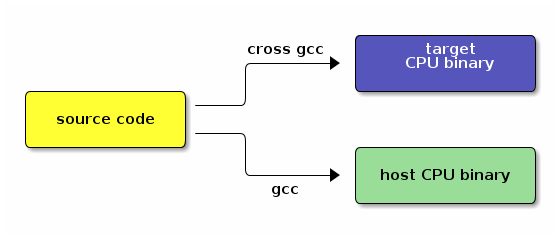
\includegraphics[scale=0.5]{cross_compile.png}
        \end{figure}
    }

    \onslide<3->
    {
        \vspace{5pt}
        => la première étape est donc de compiler le compilateur croisé.
    }
\end{frame}

%------------------------------------------------------------------------------
% cc1
%------------------------------------------------------------------------------
\begin{frame}{Compilateur croisé (1)}
    \subt{Contenu}

    \vspace{10pt}
    Une chaîne de compilation est difficile à mettre en oeuvre from scratch car
    elle contient de très nombreux éléments :

    \bi
    \itemsep6pt
    \item le compilateur en tant que tel : gcc-<ARCH>
    \item les outils fournis par GNU Binutils : ld, as, nm, ...
    \item la libc : glibc, uclibc ou eglibc
    \ei

    \onslide<2->
    {
        \vspace{10pt}
        Il existe des chaînes sur étagère, robustes et éprouvées :
        \bi
        \itemsep6pt
        \item Crosstool (vieillisant)
        \item Crosstool-NG
        \item la chaîne de ELDK
        \item la chaîne de Buildroot
        \item la chaîne de Yocto Project
        \ei
    } 

\end{frame}

%------------------------------------------------------------------------------
% cc2
%------------------------------------------------------------------------------
\begin{frame}{Compilateur croisé (2)}
    \subt{Crosstool-NG}

    \vspace{10pt}
    Auteur : Yann Morin / Fançais / ENIB.

    \onslide<2->
    {
        \vspace{10pt}
        Les architectures supportées : ARM, AVR, PPC, x86, ...
    }

    \onslide<3->
    {
        \vspace{10pt}
        À travers la configuration de Crosstool-ng, on peut choisir
        l'architecture cible, la version de gcc, la libc, la version de la
        libc, ...
    }

    \onslide<4->
    {
        \begin{figure}
            \centering
            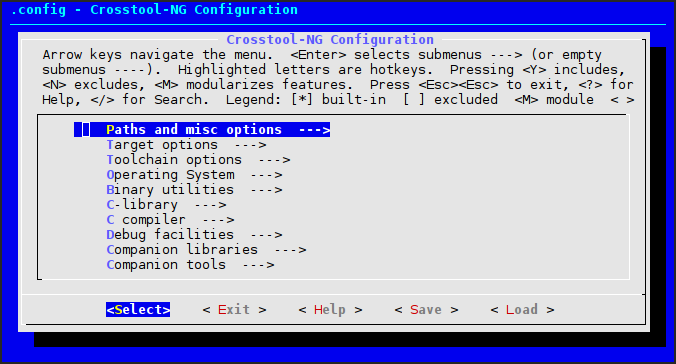
\includegraphics[scale=0.4]{ct-ng.png}
        \end{figure}
    }
\end{frame}

%------------------------------------------------------------------------------
% cc3
%------------------------------------------------------------------------------
\begin{frame}{Compilateur croisé (3)}
    \subt{ELDK}

    \vspace{15pt}
    Embedded Linux Development Kit :
    \bi
    \itemsep6pt
    \item chaîne de compilation croisée pour PPC, ARM ou MIPS
    \item distribution Linux associée à l'architecture cible
    \ei

    \onslide<2->
    {
        \vspace{15pt}
        => on peut très bien n'utiliser que la chaîne de compilation et
        construire nous même la distribution.
    }

    \onslide<3->
    {
        \vspace{15pt}
        => la chaîne de compilation de ELDK vient avec des librairies
        précompilées. On ne peut donc pas choisir les versions de gcc ou de la
        glibc
    }

    \onslide<4->
    {
        \vspace{-10pt}
        \begin{figure}
            \centering
            \hspace{140pt}
\includegraphics[scale=0.9]{denx.png}
        \end{figure}
    }
\end{frame}

%------------------------------------------------------------------------------
% cc4
%------------------------------------------------------------------------------
\begin{frame}{Compilateur croisé (4)}
    \subt{ISA et ABI}

    \vspace{5pt}
    {\textbf{Instruction Set Architecture}} : définit une interface de
    communication entre une brique logicielle et la partie matérielle.

    \onslide<2->
    {
        \vspace{5pt}
        {\textbf{Application Binary Interface}} : définit au niveau binaire une
        interface de communication entre plusieurs briques logicielles
        (librairies, OS, ...).
    }

    \onslide<3->
    {
        \begin{figure}
            \centering
            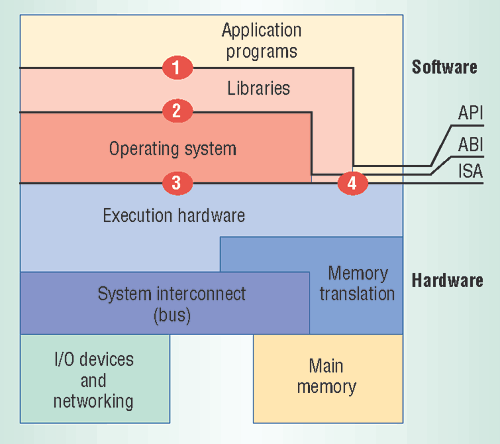
\includegraphics[scale=0.45]{abi-isa.png}
            \src{http://www.computer.org/csdl/mags/co/2005/05/r5032-abs.html}{ISA - ABI - API}
        \end{figure}
    }
\end{frame}

%------------------------------------------------------------------------------
% cc5
%------------------------------------------------------------------------------
\begin{frame}{Compilateur croisé (5)}
    \subt{ISA et ABI}

    \vspace{15pt}
    Il existe plusieurs ABI par architecture. On doit donc spécifier l'ABI
    souhaitée au moment de la compilation de la chaîne de cross-compilation!

    \onslide<2->
    {
        \vspace{15pt}
        Le choix de l'ABI a une conséquence directe sur la taille du code
        généré, l'utilisation de la mémoire, ...
    }

    \onslide<3->
    {
        \vspace{15pt}
        Par exemple pour ARM :
        \bi
        \item OABI : Old-ABI
        \item EABI : Embedded-ABI
        \ei
    }
\end{frame}

%------------------------------------------------------------------------------
% cc6
%------------------------------------------------------------------------------
\begin{frame}{Compilateur croisé (6)}
    \subt{FPU}

    \vspace{15pt}
    {\textbf{Floating Point Unit}} : unité de calcul en virgule flottante.

    \vspace{15pt}
    => dans un processeur, il peut y avoir une partie dédiée aux opérations
    sur flottant.

    \onslide<2->
    {
        \vspace{15pt}
        Si un processeur ne possède pas de FPU (dit {\textit{hardware FPU}}),
        le calcul sur nombres flottant est exécuté logiciellement par le
        compilateur lors de la génération en langage machine.

        \vspace{15pt}
        => on parle alors non pas de {\textbf{hardfpu}}, mais de
        {\textbf{softfpu}}!
    }
\end{frame}

%------------------------------------------------------------------------------
% cc7
%------------------------------------------------------------------------------
\begin{frame}{Compilateur croisé (7)}
    \subt{OABI vs EABI : un problème de FPU}

    \vspace{15pt}
    OABI part du principe que le processeur possède une FPU. Or, toutes les
    cartes sous ARM n'en possèdent pas nécessairement.

    \onslide<2->
    {
        \vspace{15pt}
        Dans le cas d'une demande d'un calcul sur flottant avec une EABI mais
        sur un processeur n'ayant pas de FPU, une exception sera levée par le
        processeur, puis attrapée par le kernel qui va lui même utiliser sa
        fonction de {\textit{softfpu}}.
    }

    \onslide <3->
    {
        \vspace{15pt}
        => terriblement inefficace car même chose sur tous les calculs sur les
        flottants!
    }
\end{frame}

%------------------------------------------------------------------------------
% cc8
%------------------------------------------------------------------------------
\begin{frame}{Compilateur croisé (8)}
    \subt{OABI vs EABI : un problème de FPU}

    \vspace{15pt}
    EABI permet de gérer la fonction de {\textit{softfpu}} dans l'espace
    utilisateur au lieu de l'espace kernel, ce qui augmente les performances.

    \vspace{15pt}
    => pour cela, il faut passer des options à gcc au moment de la compilation.
\end{frame}

%------------------------------------------------------------------------------
% cc9
%------------------------------------------------------------------------------
\begin{frame}{Compilateur croisé (9)}
    \subt{OABI vs EABI : un problème de FPU}

    \begin{figure}
        \centering
        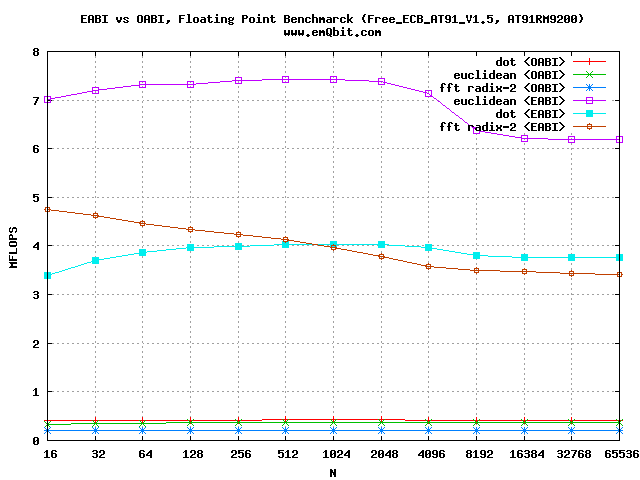
\includegraphics[scale=0.4]{benchmark.png}
        \src{http://archive.linuxgizmos.com/why-arms-eabi-matters/}{Benchmark OABI vs EABI}
    \end{figure}
\end{frame}

%------------------------------------------------------------------------------
% ker1
%------------------------------------------------------------------------------
\begin{frame}{Compilation du kernel (1)}
    \subt{Les sources}

    \vspace{10pt}
    Le code source de Linux peut être récupéré sur le github de Mr
    Torvalds : https://github.com/torvalds/linux.

    \onslide<2->
    {
        \begin{figure}
            \centering
            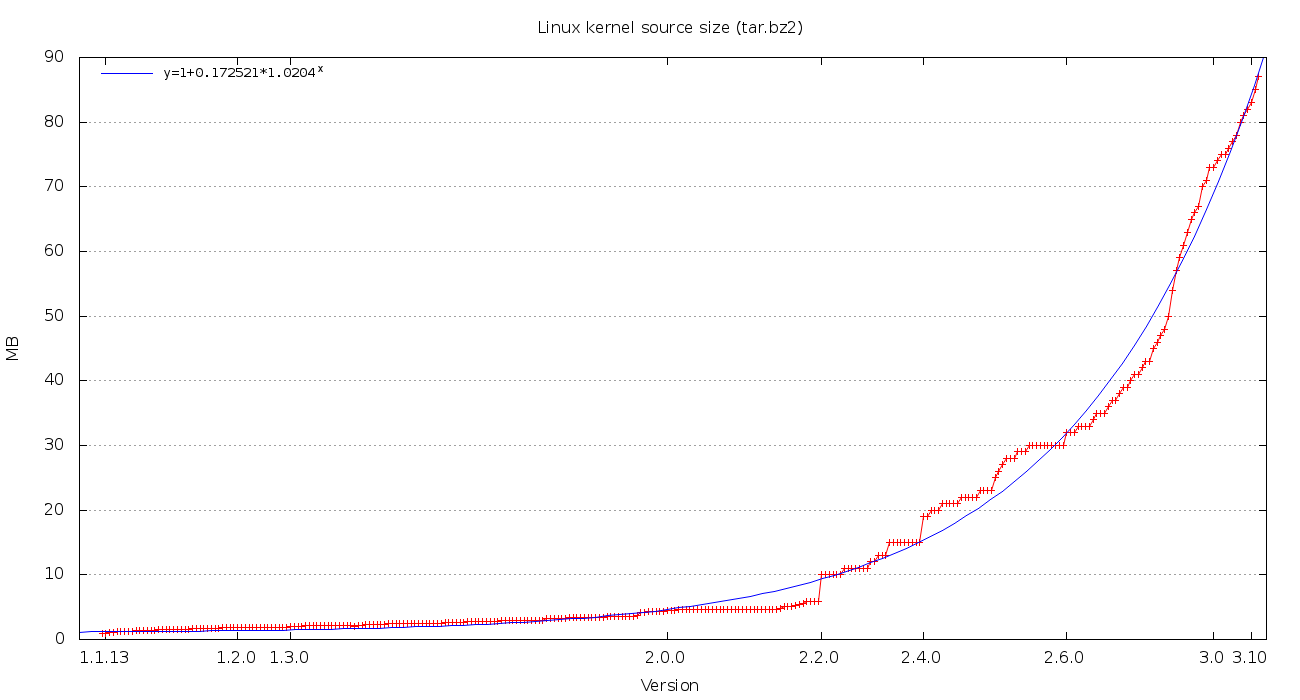
\includegraphics[scale=0.23]{kernel-size.png}
        \end{figure}
    }
\end{frame}

%------------------------------------------------------------------------------
% ker2
%------------------------------------------------------------------------------
\begin{frame}{Compilation du kernel (2)}
    \subt{Arborescence}

    \vspace{15pt}
    Les répertoires principaux :
    \bi
    \itemsep8pt
    \item arch : code spécifique aux architecture matérielles
    \item Documentation : informations au format texte
    \item drivers : les pilotes de périphériques (i2c, gpio, ...)
    \item include : les headers
    \item kernel : les sources du kernel à proprement parlé
    \item net : le code des couches réseau
    \item ...
    \ei
\end{frame}

%------------------------------------------------------------------------------
% ker3
%------------------------------------------------------------------------------
\begin{frame}{Compilation du kernel (3)}
    \subt{Les couches}

    \begin{figure}
        \centering
        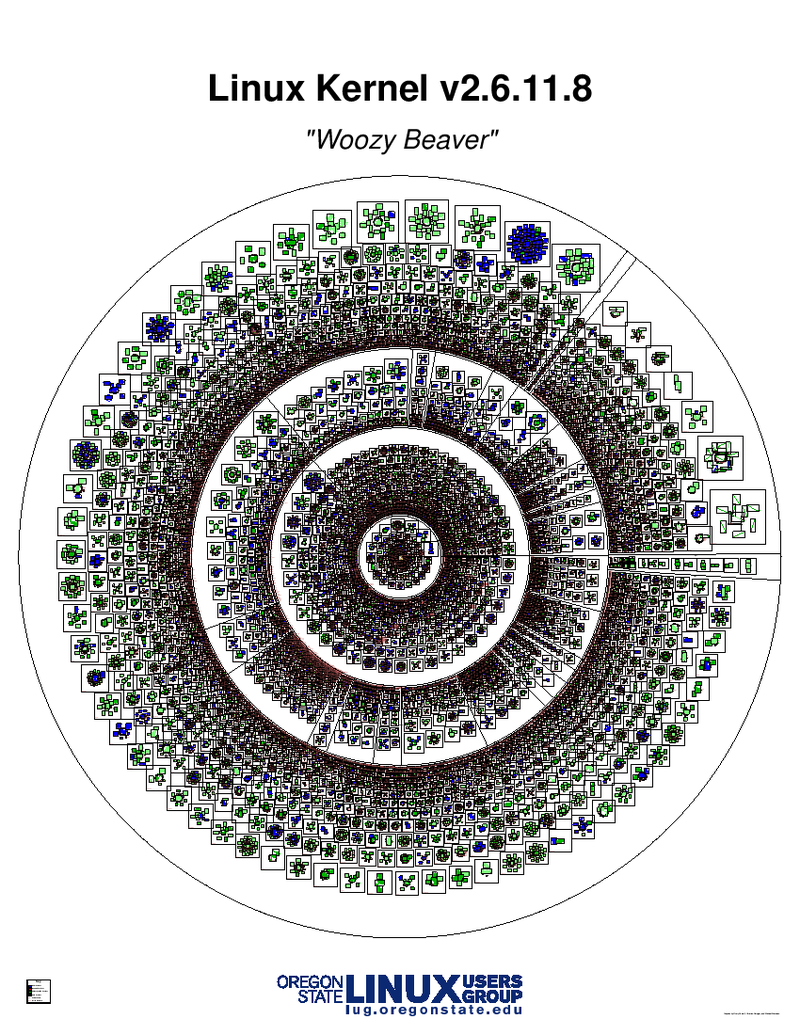
\includegraphics[scale=0.2]{kernel_onion.png}
        \src{http://keithcu.com/wordpress/?page_id=599}{Kernel sources}
    \end{figure}
\end{frame}

%------------------------------------------------------------------------------
% ker4
%------------------------------------------------------------------------------
\begin{frame}{Compilation du kernel (4)}
    \subt{Configuration}

    \vspace{15pt}
    Une configuration par défaut est disponible pour les différentes
    architectures matérielles : ce sont les fichiers <ARCH>\_defconfig.

    \onslide<2->
    {
        \vspace{15pt}
        Par exemple :
        \bi
        \itemsep10pt
        \item arch/x86/configs/i386\_defconfig
        \item arch/x86/configs/x86\_64\_defconfig
        \item arch/arm/configs/mini2440\_defconfig
        \item arch/powerpc/configs/ppc40x\_defconfig
        \ei
    }
\end{frame}

%------------------------------------------------------------------------------
% ker5
%------------------------------------------------------------------------------
\defverbatim{\lstkconf}
{
    \begin{lstlisting}
> uname -a
Linux debian 4.2.0-1-amd64 4.2.6-1 x86_64 GNU/Linux
> make sunxi_defconfig
***
*** Can't find default configuration
*** "arch/x86/configs/sunxi_defconfig"!
***
scripts/kconfig/Makefile:108: recipe for target
'sunxi_defconfig' failed
> make ARCH=arm sunxi_defconfig
#
# configuration written to .config
#
    \end{lstlisting}
}

\begin{frame}{Compilation du kernel (5)}
    \subt{Configuration}

    \vspace{10pt}
    Pour utiliser une configuration d'une architecture différente de celle
    courante :

    \vspace{10pt}
    \lstkconf

\end{frame}

%------------------------------------------------------------------------------
% ker6
%------------------------------------------------------------------------------
\defverbatim{\lstcomp}
{
    \begin{lstlisting}
> make ARCH=arm CROSS_COMPILE=/path/to/compiler
...
BUILD   arch/x86/boot/bzImage
Setup is 15708 bytes (padded to 15872 bytes).
System is 6008 kB
CRC 734d60c8
Kernel: arch/x86/boot/bzImage is ready  (#1)
    \end{lstlisting}
}

\begin{frame}{Compilation du kernel (6)}
    \subt{Compilation}

    \vspace{15pt}
    Une fois configuré, on peut compiler le kernel :
    \vspace{5pt}
    \lstcomp

    \onslide<2->
    {
        \vspace{5pt}
        => le fichier {\textbf{bzImage}} est la partie statique du kernel!
    }
\end{frame}

%------------------------------------------------------------------------------
% ker7
%------------------------------------------------------------------------------
\defverbatim{\lstmod}
{
    \begin{lstlisting}
> mkdir fake_rfs
> make modules_install INSTALL_MOD_PATH=./fake_rfs
scripts/kconfig/conf  --silentoldconfig Kconfig
INSTALL crypto/echainiv.ko
INSTALL drivers/thermal/x86_pkg_temp_thermal.ko
...
INSTALL net/netfilter/xt_nat.ko
DEPMOD  4.4.0-rc5
> ls fake_rfs/lib/modules/4.4.0-rc5/
... kernel ... modules.alias modules.dep ...
> ls fake_rfs/lib/modules/4.4.0-rc5/kernel/
crypto  drivers  fs  net
    \end{lstlisting}
}

\begin{frame}{Compilation du kernel (7)}
    \subt{Les modules}

    \vspace{10pt}
    Les modules (fichiers .ko) doivent être installés sur un RFS :
    \vspace{5pt}
    \lstmod

\end{frame}

%------------------------------------------------------------------------------
% busybox
%------------------------------------------------------------------------------
\begin{frame}{Busybox (1)}
    \subt{Qu'est ce?}

    \vspace{15pt}
    Dans le cadre d'un système embarqué, l'environnement d'outils et
    d'applications fournis à travers le RFS doit :
    \bi
    \itemsep8pt
    \item être de volume réduit
    \item avoir une consommation en ressources réduite
    \item être portable sur diverses architectures matérielles
    \ei

    \onslide<2->
    {
        \vspace{10pt}
        => pour cela, le projet Busybox est utilisé dans quasiment tous les
        équipements basés sur des distributions customisées.

        \begin{figure}
            \centering
            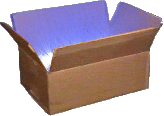
\includegraphics[scale=0.5]{busybox.png}
        \end{figure}
    }
\end{frame}

%------------------------------------------------------------------------------
% busybox2
%------------------------------------------------------------------------------
\begin{frame}{Busybox (2)}
    \subt{Configuration}

    \vspace{15pt}
    La configuration de Busybox utilise aussi KConfig et est disponible grâce
    à la commande {\textbf{make menuconfig}}.

    \onslide<2->
    {
        \begin{figure}
            \centering
            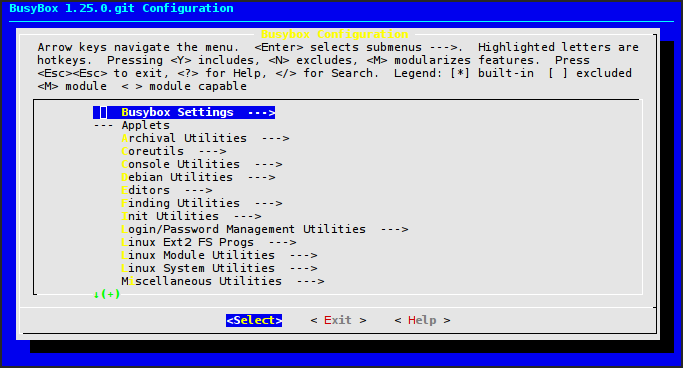
\includegraphics[scale=0.5]{busybox_conf.png}
        \end{figure}
    }
\end{frame}

%------------------------------------------------------------------------------
% busybox3
%------------------------------------------------------------------------------
\defverbatim{\lstbusyinst}
{
    \begin{lstlisting}
> make ARCH=arm CROSS_COMPILE=/path/to/binary
HOSTCC  scripts/basic/fixdep
HOSTCC  scripts/basic/split-include
HOSTCC  scripts/basic/docproc
...
DOC     BusyBox.txt
DOC     busybox.1
DOC     BusyBox.html
> mkdir fake_rfs
> make install CONFIG_PREFIX=./fake_rfs/
./fake_prefix///bin/ash -> busybox
./fake_prefix///bin/base64 -> busybox
...
\end{lstlisting}
}

\begin{frame}{Busybox (3)}
    \subt{Installation}

    \vspace{15pt}
    Pour la compilation et l'installation :
    \vspace{5pt}
    \lstbusyinst

\end{frame}

%------------------------------------------------------------------------------
% busybox4
%------------------------------------------------------------------------------
\defverbatim{\lstbusyres}
{
    \begin{lstlisting}
> ls fake_rfs
total 820
  drwxr-xr-x 2 4096 Dec 21 18:01 .
  drwxr-xr-x 5 4096 Dec 21 18:01 ..
  lrwxrwxrwx 1 7 Dec 21 18:01 ash -> busybox
  l-rwxr-xr-x 1 829680 Dec 21 18:01 busybox
  lrwxrwxrwx 1 7 Dec 21 18:01 cat -> busybox
  lrwxrwxrwx 1 7 Dec 21 18:01 base64 -> busybox
  ...
    \end{lstlisting}
}

\begin{frame}{Busybox (4)}
    \subt{Liens symboliques}

    \vspace{15pt}
    \lstbusyres

    \onslide<2->
    {
        \vspace{5pt}
        => busybox est un binaire unique fournissant les commandes grâce à un jeu
        de liens symboliques
    }

    \onslide<3->
    {
        \vspace{5pt}
        => la taille du binaire est limitée par mutualisation des fonctions
        communes
    }
\end{frame}

%------------------------------------------------------------------------------
% uboot1
%------------------------------------------------------------------------------
\begin{frame}{U-Boot (1)}
    \subt{Les bootloaders}

    \vspace{15pt}
    Un bootloader est notamment chargé d'exécuter le kernel et est capable
    d'utiliser les fonctions matérielles de base :

    \bi
    \itemsep8pt
    \item la mémoire vive et mémoire flash
    \item les ports série
    \item le réseau filaire (Ethernet)
    \ei

    \onslide<2->
    {
        \vspace{15pt}
        Pour les plateformes x86, GRUB est généralement utilisé.

        \begin{figure}
            \centering
            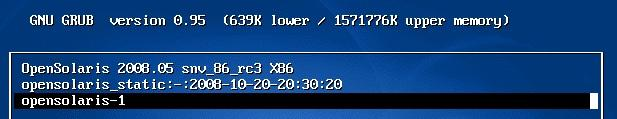
\includegraphics[scale=0.5]{grub-menu.jpg}
        \end{figure}
    }
\end{frame}

%------------------------------------------------------------------------------
% uboot2
%------------------------------------------------------------------------------
\begin{frame}{U-Boot (2)}
    \subt{JTAG}

    \vspace{15pt}
    L'installation d'un bootloader sur carte peut être réalisée par liaison
    série (si un bootloader est déjà présent) ou bien par JTAG : {\textbf{Join
    Test Action Group}}.

    \onslide<2->
    {
        \vspace{15pt}
        => l'installation du bootloader est une étape critique et peut rendre une
        carte inutilisable!
    }
\end{frame}

%------------------------------------------------------------------------------
% uboot3
%------------------------------------------------------------------------------
\begin{frame}{U-Boot (3)}
    \subt{JTAG et Raspberry Pi}

    \vspace{15pt}
    \begin{figure}
        \centering
        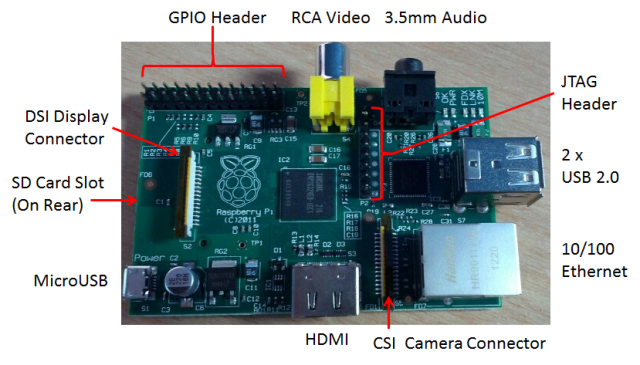
\includegraphics[scale=0.5]{rpi_jtag.png}
    \end{figure}
\end{frame}

%------------------------------------------------------------------------------
% uboot4
%------------------------------------------------------------------------------
\begin{frame}{U-Boot (4)}
    \subt{JTAG et Xbox 360}

    \vspace{15pt}
    Un hack connu de la Xbox 360 est d'ajouter la possibilité de lire des jeux
    sur disque dur, clé USB ou par FTP.

    \onslide<2->
    {
        \vspace{15pt}
        Pour cela, il faut se connecter sur le port JTAG de la carte mère et
        charger une nouvelle image NAND!

        \begin{figure}
            \centering
            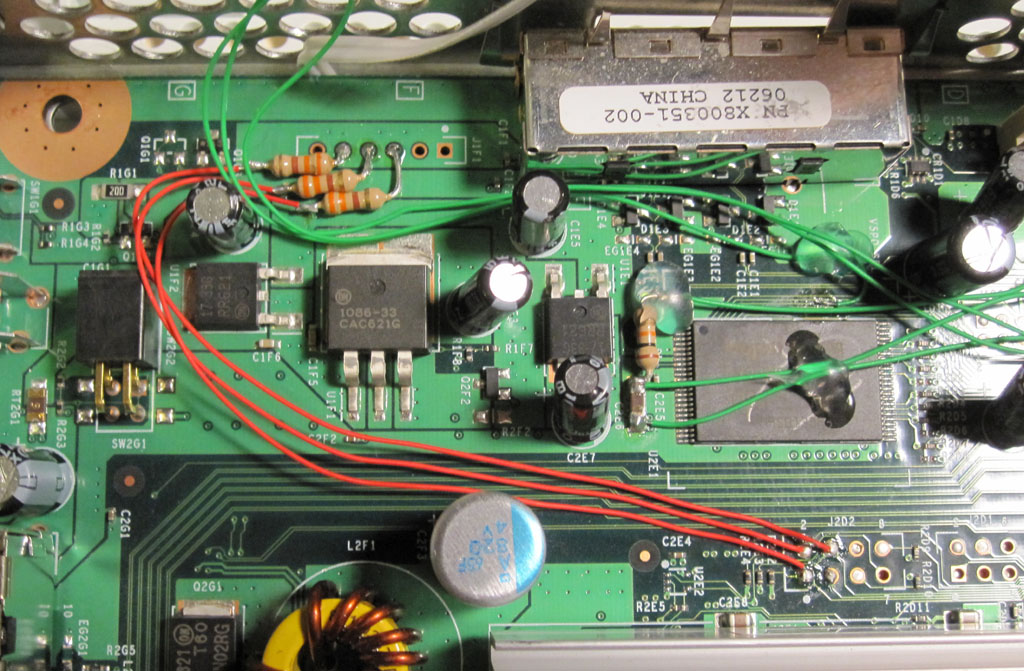
\includegraphics[scale=0.7]{xbox_jtag.jpg}
        \end{figure}
    }
\end{frame}

%------------------------------------------------------------------------------
% uboot5
%------------------------------------------------------------------------------
\begin{frame}{U-Boot (5)}
    \subt{TFTP}

    \vspace{15pt}
    {\textbf{Trivial File Transfert Protocol}} : connexion UDP (port 69 par
    défaut) permettant le transfert de fichiers.

    \onslide<2->
    {
        \begin{figure}
            \centering
            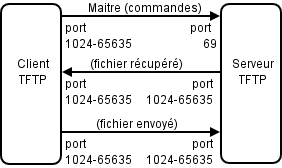
\includegraphics[scale=0.4]{tftp.png}
        \end{figure}
    }

    \onslide<3->
    {
        => très utilisé en embarqué!
    }
\end{frame}

%------------------------------------------------------------------------------
% uboot6
%------------------------------------------------------------------------------
\begin{frame}{U-Boot (6)}
    \subt{Universal Bootloader}

    \vspace{15pt}
    Dans le monde de l'embarqué, en dehors des cartes x86, U-Boot est le
    bootloader le plus répandu.

    \onslide<2->
    {
        \vspace{15pt}
        Utilisation classique :
        \bi
        \itemsep8pt
        \item connexion à la carte par liaison série et accès au prompt U-Boot
        \item configuration du server TFTP
        \item téléchargement de l'image kernel et du RFS par TFTP et écriture
              sur mémoire flash
        \item modification de la commande de démarrage
        \item boot
        \ei
    }
\end{frame}

%------------------------------------------------------------------------------
% uboot7
%------------------------------------------------------------------------------
\begin{frame}{U-Boot (7)}
    \subt{prompt}

    \vspace{15pt}
    Le prompt de U-Boot offre de très nombreuses commandes et permet
    d'enregistrer sur la flash des variables d'environnement.

    \onslide<2->
    \vspace{5pt}
        \begin{figure}
            \centering
            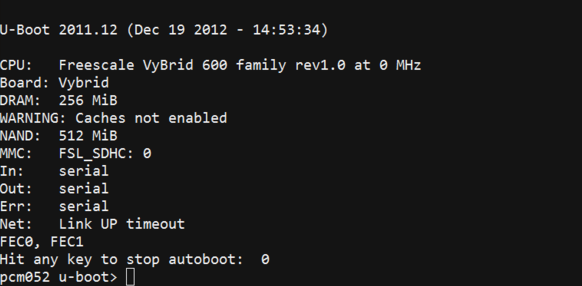
\includegraphics[scale=0.8]{uboot_prompt.png}
        \end{figure}

\end{frame}

%------------------------------------------------------------------------------
% uboot8
%------------------------------------------------------------------------------
\begin{frame}{U-Boot (8)}
    \subt{Commandes et variables d'environnement}

    \vspace{5pt}
    Liste non exhaustive :
    \vspace{10pt}
    \bi
    \itemsep6pt
    \item {\textbf{run}} : exécution d'une macro
    \item {\textbf{bootm}} : démarrage d'une image stockée en mémoire
    \item {\textbf{bootcmd}} : macro de démarrage (exécutée automatiquement
          quand {\textbf{bootdelay}} arrive à 0 en autoboot)
      \item {\textbf{boot}} : équivaut à {\textbf{run bootcmd}}
    \item {\textbf{setenv}} : affectation d'une variable d'environnement
    \item {\textbf{saveenv}} : sauvegarde de l'environnement sur la flash
    \item {\textbf{printenv}} : affichage des variables d'environnement et des
          macros
    \ei

\end{frame}

%------------------------------------------------------------------------------
% auto1
%------------------------------------------------------------------------------
\begin{frame}{Automatisation (1)}
    \subt{Buildroot}

    \vspace{15pt}
    Buildroot est un ensemble de Makefile automatisant le process de build
    d'une distribution Linux embarquée.

    \onslide<2->
    {
        \vspace{15pt}
        Pour la phase de cross-compilation, soit Buildroot en construit une, soit
        on lui indique d'utiliser une chaîne custom (comme celle de Crosstool-ng).
    }

    \onslide<3->
    {
        \vspace{15pt}
        Configurable à la {\textit{menuconfig}}.
    }

    \onslide<4->
    {
        \vspace{10pt}
        \begin{figure}
            \centering
            
\includegraphics[scale=0.35]{logo-buildroot.png}
        \end{figure}
    }
\end{frame}

%------------------------------------------------------------------------------
% auto2
%------------------------------------------------------------------------------
\begin{frame}{Automatisation (2)}
    \subt{Buildroot}

    \begin{figure}
        \vspace{-23pt}
        \hspace{30pt}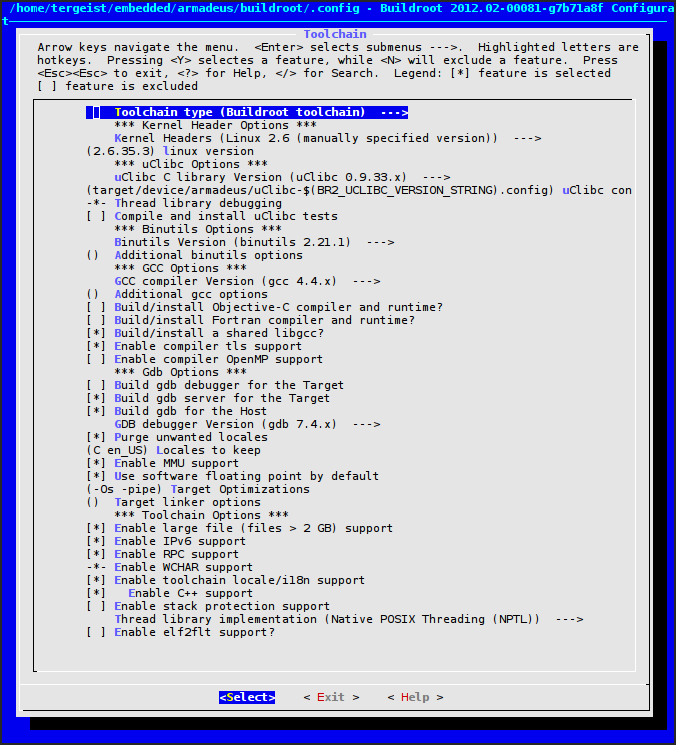
\includegraphics[scale=0.5]{buildroot_sc.png}
    \end{figure}

\end{frame}

%------------------------------------------------------------------------------
% auto3
%------------------------------------------------------------------------------
\begin{frame}{Automatisation (3)}
    \subt{Buildroot}

    \vspace{15pt}
    Les répertoires principaux :
    \bi
    \itemsep10pt
    \item {\textbf{configs}} : fichiers de configuration pour la compilation
    \item {\textbf{downloads}} : les archives téléchargées sont ici
    \item {\textbf{output/build}} : les paquets et librairies compilés
    \item {\textbf{output/host}} : chaîne de cross-compilation
    \item {\textbf{output/images}} : les images compilées
    \item {\textbf{package}} : les règles de compilation
    \ei
\end{frame}

%------------------------------------------------------------------------------
% auto4
%------------------------------------------------------------------------------
\begin{frame}{Automatisation (4)}
    \subt{Buildroot}

    \vspace{15pt}
    Les options principales du make :
    \bi
    \itemsep10pt
    \item {\textbf{clean}} : nettoie tout ce qui a été compilé
    \item {\textbf{toolchain}} : contruit seulement la chaîne de compilation
          croisée
    \item {\textbf{busybox-menuconfig}} : configuration de busybox
    \item {\textbf{uclibc-menuconfig}} : configuration de la uclibc
    \item {\textbf{linux-menuconfig}} : configuration du kernel
    \ei

\end{frame}

%------------------------------------------------------------------------------
% auto3
%------------------------------------------------------------------------------
\defverbatim{\lststamp}
{
    \begin{lstlisting}
> cd output/build/busybox-1.23.1
> ls .stamp_*
.stamp_built      .stamp_downloaded .stamp_patched
.stamp_configured .stamp_extracted  .stamp_installed
    \end{lstlisting}
}

\begin{frame}{Automatisation (4)}
    \subt{Buildroot}

    \vspace{15pt}
    Buildroot créé des fichiers {\textit{.stamp\_}} pour se repérer dans
    les étapes de construction/compilation :
    \vspace{10pt}
    \lststamp

    \begin{figure}
        
\includegraphics[scale=0.3]{done.png}
    \end{figure}

\end{frame}

%------------------------------------------------------------------------------
% auto4
%------------------------------------------------------------------------------
\begin{frame}{Automatisation (4)}
    \subt{Yocto Project}

    \vspace{20pt}
    Système de build long à prendre en main mais offrant davantage de
    fonctionnalités que Buildroot.

    \vspace{20pt}
    À la mode!

    \vspace{20pt}
    \begin{figure}
        
\includegraphics[scale=1]{yocto.png}
    \end{figure}

\end{frame}

%------------------------------------------------------------------------------
% qemu1
%------------------------------------------------------------------------------
\begin{frame}{QEMU (1)}
    \subt{Principe}

    \vspace{10pt}
    Émulateur de matériel permettant de simuler des architectures différentes de
    celle courante : x86, PPC, ARM SPARC.

    \begin{figure}
        
\includegraphics[scale=0.5]{qemu.png}
    \end{figure}

    \onslide<2->
    {
        \vspace{5pt}
        Très utilisé en embarqué car permet de tester les images compilées (kernel,
        rootfs et uboot) directement sur la machine de travail :
        \bi
        \itemsep6pt
        \item gain de temps important
        \item facilité d'utilisation
        \item permet de se passer du matériel pour la phase de mise au point
        \ei
    }
\end{frame}

%------------------------------------------------------------------------------
% qemu2
%------------------------------------------------------------------------------
\defverbatim{\lstqemu}
{
    \begin{lstlisting}
> qemu-system-arm -M versatilepb -m 128M -kernel \
  uImage -initrd rootfs
    \end{lstlisting}
}

\begin{frame}{QEMU (2)}
    \subt{Utilisation}

    \vspace{15pt}
    Il existe un binaire {\textbf{qemu-system-<ARCH>}} pour chaque architecture
    supportée : qemu-system-arm, qemu-system-ppc, qemu-system-x86\_64, ...

    \onslide<2->
    {
        \vspace{15pt}
        Les options principales :
        \vspace{5pt}
        \bi
        \itemsep6pt
        \item {\textbf{-M}} : machine à émuler
        \item {\textbf{-m}} : quantité de RAM
        \item {\textbf{-kernel}} : image kernel à utiliser
        \item {\textbf{-initrd}} : ramdisk
        \ei
    }

    \onslide<3->
    {
        \vspace{15pt}
        \lstqemu
    }
\end{frame}

%------------------------------------------------------------------------------
% concl1
%------------------------------------------------------------------------------
\begin{frame}{Conclusion}

    \centering
    \vspace{20pt}
    \LARGE{
        Il existe de très nombreux outils dans le monde des systèmes embarqués.
        Le tout est simplement de s'y retrouver!

        \begin{figure}
            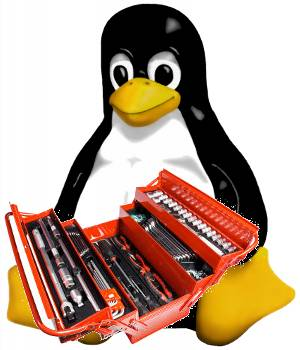
\includegraphics[scale=0.25]{tux-toolbox.jpg}
        \end{figure}
    }

\end{frame}

%------------------------------------------------------------------------------
% ref
%------------------------------------------------------------------------------
\begin{frame}{Références}
    \vspace{30pt}

    \bi
    \itemsep12pt
    \item Free Electrons
    \item Linux Embarqué - Pierre Ficheux
    \ei

\end{frame}
%<//lecture_content>

\end{document}
